\chapter{Evaluare}
\section{Modalitatea de construire a testelor}
Pentru evaluarea opera'tiilor structurilor de AVL Tree 'si Max - Heap s-au implementat 'in etapa trecut'a c\^ate 5 teste care au fost construite folosind un generator de numere distincte\cite{Random} 'si un instrument de sortare online\cite{Endmemo}, numerele fiind generate 'intr-o ordine aleatoare 'si mai mici de 1000. Aceste teste au un num'ar de 5, 10, 25, 50 'si 100 de elemente distincte. Pentru o mai bun'a acurate'te a performan'tei opera'tiilor se vor mai ad'auga un set de 5 teste pentru fiecare structur'a. Un test va fi de 250 de elemente generate 'in ordine aleatoare, dou'a teste vor fi de 500 'si 1000 de elemente 'si vor fi generate descresc'ator, iar celelalte dou'a teste vor fi de 5000 'si 10000 de elemente generate cresc'ator.
\myindent Fiecare test va rula toate opera'tiile structurii de date reprezentate. Pentru AVL se vor executa: Crearea structurii, Inserarea elementelor, C'autarea maximului 'si minimului, Eliminarea maximului 'si minimului din structur'a 'si 'Stergerea structurii, iar pentru Heap se vor executa: Crearea structurii, Inserarea elementelor, Preluarea nodului cu valoare maxim'a, Extrgerea nodului cu valoare maxim'a 'si 'stergerea structurii.
\vspace{5 mm}
\section{Rezultatele testelor}
\begin{table}[ht]
\centering
\caption{Timpii de execu'tie pentru crearea structurilor}
\begin{tabular}{| p{5cm} | p{5cm} | p{5cm} |}
\hline
N & AVL Tree & Max - Heap \\
\hline\hline
5 & 0.001178 ms & 0.001106 ms \\
\hline
10 & 0.000726 ms & 0.001051 ms \\
\hline
25 & 0.000682 ms & 0.000986 ms \\
\hline
50 & 0.000677 ms & 0.00114 ms \\
\hline
100 & 0.000676 ms & 0.002253 ms \\
\hline
250 & 0.000707 ms & 0.003481 ms \\
\hline
500 & 0.000898 ms & 0.005623 ms \\
\hline
1000 & 0.000984 ms & 0.010363 ms \\
\hline
5000 & 0.000797 ms & 0.04761 ms \\
\hline
10000 & 0.000861 ms & 0.362846 ms \\
\hline
\end{tabular}
\end{table}
\FloatBarrier

\begin{figure}[ht]
\centering
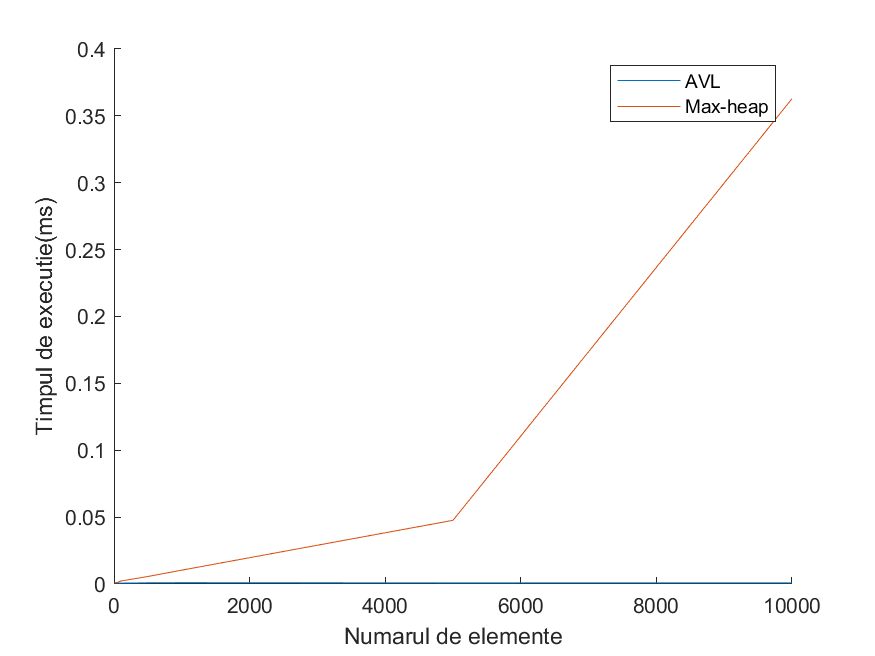
\includegraphics[scale=0.8]{Fisiere/creare}
\caption {Diagrama pentru crearea structurilor}
\end{figure}
\FloatBarrier

\begin{table}[ht]
\centering
\caption{Timpii de execu'tie pentru inserarea elementelor}
\begin{tabular}{| p{5cm} | p{5cm} | p{5cm} |}
\hline
N & AVL Tree & Max - Heap \\
\hline\hline
5 & 0.001159 ms & 0.010295 ms \\
\hline
10 & 0.017719 ms & 0.010691 ms \\
\hline
25 & 0.041883 ms & 0.02151 ms \\
\hline
50 & 0.096804 ms & 0.052967 ms \\
\hline
100 & 0.221705 ms & 0.109183 ms \\
\hline
250 & 0.591891 ms & 0.225686 ms \\
\hline
500 & 1.29952 ms & 0.379961 ms \\
\hline
1000 & 3.05291 ms & 0.692936 ms \\
\hline
5000 & 19.6206 ms & 11.6697 ms \\
\hline
10000 & 59.8021 ms & 24.26 ms \\
\hline
\end{tabular}
\end{table}
\FloatBarrier

\begin{figure}[ht]
\centering
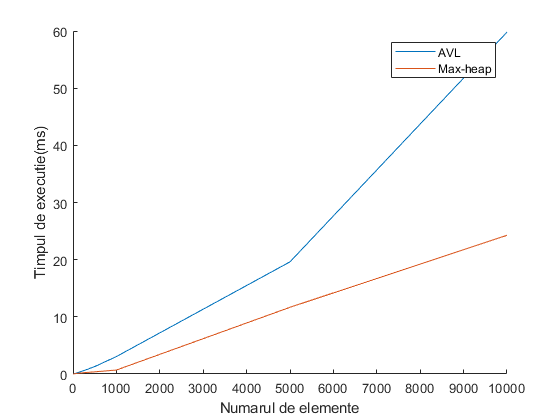
\includegraphics[scale=0.8]{Fisiere/inserare}
\caption {Diagrama pentru inserarea elementelor}
\end{figure}
\FloatBarrier

\vspace{5 mm}
\begin{table}[ht]
\centering
\caption{Timpii de execu'tie pentru g'asirea elementelor maxime}
\begin{tabular}{| p{5cm} | p{5cm} | p{5cm} |}
\hline
N & AVL Tree & Max - Heap \\
\hline\hline
5 & 0.007937 ms & 0.000431 ms \\
\hline
10 & 0.008015 ms & 0.000409 ms \\
\hline
25 & 0.008226 ms & 0.000412 ms \\
\hline
50 & 0.008193 ms & 0.000427 ms \\
\hline
100 & 0.008362 ms & 0.00044 ms \\
\hline
250 & 0.008447 ms & 0.000453 ms \\
\hline
500 & 0.010743 ms & 0.000468 ms \\
\hline
1000 & 0.01005 ms & 0.000466 ms \\
\hline
5000 & 0.011588 ms & 0.000485 ms \\
\hline
10000 & 0.012177 ms & 0.000631 ms \\
\hline
\end{tabular}
\end{table}
\FloatBarrier

\begin{figure}[ht]
\centering
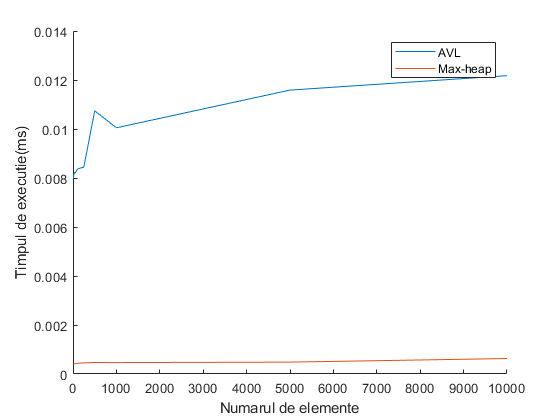
\includegraphics[scale=0.8]{Fisiere/FindMax}
\caption {Diagrama pentru g'asirea elementelor maxime}
\end{figure}
\FloatBarrier

\vspace{5 mm}
\begin{table}[ht]
\centering
\caption{Timpii de execu'tie pentru eliminarea elementelor maxime}
\begin{tabular}{| p{5cm} | p{5cm} | p{5cm} |}
\hline
N & AVL Tree & Max - Heap \\
\hline\hline
5 & 0.000388 ms & 0.000667 ms \\
\hline
10 & 0.000677 ms & 0.000737 ms \\
\hline
25 & 0.000573 ms & 0.001418 ms \\
\hline
50 & 0.000555 ms & 0.001529 ms \\
\hline
100 & 0.00108 ms & 0.001674 ms \\
\hline
250 & 0.001119 ms & 0.001795 ms \\
\hline
500 & 0.000832 ms & 0.001991 ms \\
\hline
1000 & 0.000983 ms & 0.002041 ms \\
\hline
5000 & 0.005285 ms & 0.00266 ms \\
\hline
10000 & 0.00594 ms & 0.002867 ms \\
\hline
\end{tabular}
\end{table}
\FloatBarrier

\begin{figure}[ht]
\centering
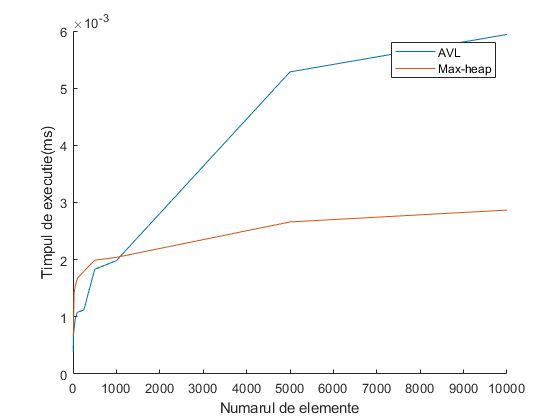
\includegraphics[scale=0.8]{Fisiere/DelMax}
\caption {Diagrama pentru eliminarea elementelor maxime}
\end{figure}
\FloatBarrier

\begin{table}[ht]
\centering
\caption{Timpii de execu'tie pentru 'stergerea structurii}
\begin{tabular}{| p{5cm} | p{5cm} | p{5cm} |}
\hline
N & AVL Tree & Max - Heap \\
\hline\hline
5 & 0.000501 ms & 0.000473 ms \\
\hline
10 & 0.000808 ms & 0.000328 ms \\
\hline
25 & 0.001794 ms & 0.000268 ms \\
\hline
50 & 0.003458 ms & 0.000297 ms \\
\hline
100 & 0.007003 ms & 0.000362 ms \\
\hline
250 & 0.013364 ms & 0.000416 ms \\
\hline
500 & 0.02463 ms & 0.000444 ms \\
\hline
1000 & 0.04781 ms & 0.00032 ms \\
\hline
5000 & 0.369463 ms & 0.00076 ms \\
\hline
10000 & 0.753662 ms & 0.00088 ms \\
\hline
\end{tabular}
\end{table}
\FloatBarrier

\begin{figure}[ht]
\centering
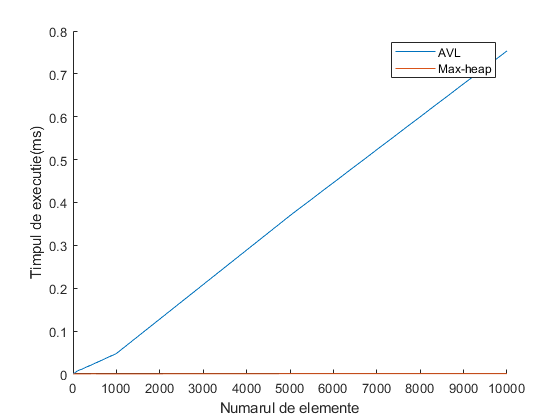
\includegraphics[scale=0.8]{Fisiere/Del}
\caption {Diagrama pentru 'stergerea structurilor}
\end{figure}
\FloatBarrier

\section{Prezentarea rezultatelor testelor}
Pentru crearea structurii propriu-zise se poate observa c'a AVL-ul are pentru orice set de date o eficien't'a mult mai bun'a din punctul de vedere al timpului de execu'tie fa't'a de Max-Heap, 'ins'a diferen'ta nu este foarte mare. Pentru Insert pentru teste sub 1000 de elemente structurile sunt la fel de eficiente, ins'a pentru teste mai mari Max - Heap - ul este mult mai bun fa't'a de AVL. Pentru g'asirea elementului maxim Max-Heap-ul av\^and valoarea maxim'a in nodul r'ad'acin'a este clar c'a v'a scoate timpi foarte mici de execu'tie datorit'a complexit'a'tii O(1) care 'in compara'tie cu O(log n) este diferen't'a semnificativ'a in special la seturi foarte mari de date. Pentru eliminarea elementului maxim AVL-ul este mai eficient dec\^at Max Heap-ul pentru input-uri mai mici de 1200 de elemente, 'insa pentru testele mai mari Max-Heap-ul este mai bun. 'In final, pentru 'stergerea structurilor, Max-Heap-ul are o performan't'a mult mai bun'a 'in compara'tie cu AVL.

\section{Specifica'tiile sistemului de calcul}
Tema a fost implementat'a folosind C++, compilat'a folosind G++ versiunea 9.3.0 'si a fost rulat'a pe o masin'a virtual'a cu Ubuntu 20.04 cu 6GB RAM aloca'ti. Configura'tia host-ului este Windows 10 cu Procesor Intel Core i7-5500U cu 2 core-uri de 2,4 GHZ, 16 GB RAM 'si plac'a Video NVidia cu 2GB.